% Provenance (never printed): see sources/outline_sources.md (Year 2: Hadean, Archean and
% Proterozoic; early crust and greenstone belts; the oxygenation of the atmosphere; snowball
% Earth). Eons and eras from the ICS chart; greenstone belts, TTG and cratons after Cawood and
% others (2018) and Smithies and others (2019); komatiite liquidus after Sossi and O'Neill (2016),
% Pierru and others (2022) and Asimow (2022); the Archean air and the GOE after Catling and Zahnle
% (2020) and Luo and others (2016); the boring billion after Lyons and others (2021); snowball
% Earth after Hoffman and others (2017). The energy-balance model, the komatiite line and the CO2
% build-up from figdata/bachelor-2/precambrian.py; exercise and problem values in the Book 4
% scratch calculator calc/ch18.py.
\chapter{A Terra pré-cambriana}\label{ch:b2:precambrian-earth}

Os primeiros fósseis com concha aparecem em rochas de cerca de 540 milhões de anos. Tudo o que vem antes deles, desde
o nascimento da Terra, há \qty{4567}{Ma}, é o Pré-Cambriano: sete oitavos da história do
planeta. Nesse tempo a Terra construiu os núcleos de seus continentes, encheu seu ar de oxigênio
e pelo menos duas vezes congelou dos polos ao equador, com mantos de gelo chegando ao mar
nos trópicos. Este capítulo lê esses quatro bilhões de anos nas rochas que restam deles
e põe números em três de seus enigmas: por que as lavas mais antigas eram tão quentes, como um
planeta congelado pode degelar e como a Terra jovem se manteve quente sob um Sol fraco.
% ledger: ics:base.Hadean, ics:base.Phanerozoic, hoffman17:cryochrons

\begin{recall}
\textbf{Dos volumes escolares}: a idade da Terra; os éons da escala do tempo geológico;
a lei de luminosidade do Sol jovem e o \omterm{def:b2:precambrian-earth:faint-sun}{problema do Sol jovem fraco}; a atmosfera primitiva;
os estromatólitos, as \omterm{def:b2:precambrian-earth:bif}{formações ferríferas bandadas}, o \omterm{def:b2:precambrian-earth:goe}{Grande Evento de Oxidação} e as camadas vermelhas; os \omterm{def:b2:precambrian-earth:craton}{crátons};
o calor radiogênico no passado. \textbf{Do volume do primeiro ano}: o zircão e suas idades U--Pb,
a temperatura de fechamento; a produção de calor radiogênico dos quatro isótopos; a radiação de onda
longa emitida e a insolação média global $S_0/4$; as unidades cronoestratigráficas.
\textbf{Dos capítulos anteriores}: a \omterm{def:b2:mantle-melting:tp}{temperatura potencial do manto} e a adiabática
(\cref{ch:b2:mantle-melting}); o liquidus e a \omterm{def:b2:magmatic-differentiation:crystallisation}{cristalização fracionada} da olivina
(\cref{ch:b2:magmatic-differentiation}); os tipos de granito (\cref{ch:b2:crustal-melting});
os \omterm{def:b2:wilson-cycle:supercontinent}{supercontinentes} (\cref{ch:b2:wilson-cycle}). A oxidação e a redução pertencem aos livros
de química, e os primeiros eucariontes e a fotossíntese aos livros de biologia.
\end{recall}

\section{Três éons antes dos fósseis}\label{sec:b2:precambrian-earth:eons}

\begin{definition}[Hadeano, Arqueano, Proterozoico]\label{def:b2:precambrian-earth:eons}
O tempo anterior ao Fanerozoico divide-se em três éons. O \emph{Hadeano}\index{Hadeano}
vai da formação da Terra, há \qty{4567}{Ma}, até $4031 \pm \qty{3}{Ma}$; o
\emph{Arqueano}\index{Arqueano}, de $4031$ a \qty{2500}{Ma}; o
\emph{Proterozoico}\index{Proterozoico}, de 2500 a \qty{538.8}{Ma}, a base do Cambriano.
Juntos, são chamados informalmente de Pré-Cambriano.
\end{definition}
% ledger: ics:base.Hadean, ics:base.Archean, ics:base.Proterozoic, ics:base.Phanerozoic

O \omterm{def:b2:precambrian-earth:eons}{Arqueano} divide-se em quatro eras, o Eoarqueano (4031 a \qty{3600}{Ma}), o Paleoarqueano (3600
a 3200), o Mesoarqueano (3200 a 2800) e o Neoarqueano (2800 a 2500); o \omterm{def:b2:precambrian-earth:eons}{Proterozoico}, em três,
o Paleoproterozoico (2500 a \qty{1600}{Ma}), o Mesoproterozoico (1600 a 1000) e o
Neoproterozoico (1000 a 538.8). Dois períodos do Neoproterozoico importam adiante, o Criogeniano, de 720 a
\qty{635}{Ma}, e o Ediacarano, de 635 a \qty{538.8}{Ma}.
% ledger: ics4:archean-eras, ics4:proterozoic-eras

\begin{omfigure}
\centering
% ledger: ics:base.Hadean, ics:base.Archean, ics:base.Proterozoic, ics:base.Phanerozoic, ics4:archean-eras, ics4:proterozoic-eras, wilde01:4404, bowring99:acasta, cz20:impacts, allwood06:spc, cawood18:transition, gumsley17:goe, luo16:goe, hoffman17:earlier, earle:bif, lyons21:boring, hoffman17:ages, asimow22:komatiite
\begin{tikzpicture}[x=-3.4cm, y=1cm, font=\scriptsize]
% eons
\fill[icsHadean] (4.567,0) rectangle (4.031,0.5);
\fill[icsArchean] (4.031,0) rectangle (2.5,0.5);
\fill[icsProterozoic] (2.5,0) rectangle (0.5388,0.5);
\fill[icsPhanerozoic] (0.5388,0) rectangle (0,0.5);
\node[text=white] at (4.299,0.25) {Hadeano};
\node[text=white] at (3.27,0.25) {Arqueano};
\node[text=white] at (1.52,0.25) {Proterozoico};
\node at (0.27,0.25) {Fan.};
% eras
\foreach \a/\b/\c in {4.031/3.6/35, 3.6/3.2/55, 3.2/2.8/35, 2.8/2.5/55}
  \fill[icsArchean!\c] (\a,-0.45) rectangle (\b,0);
\foreach \a/\b/\c in {2.5/1.6/35, 1.6/1.0/55, 1.0/0.5388/35}
  \fill[icsProterozoic!\c] (\a,-0.45) rectangle (\b,0);
\foreach \x/\l in {3.8155/Eo, 3.4/Paleo, 3.0/Meso, 2.65/Neo, 2.05/Paleo, 1.3/Meso, 0.769/Neo}
  \node at (\x,-0.225) {\l};
% axis
\draw (4.6,-0.6) -- (0,-0.6);
\foreach \t in {0,0.5,...,4.5} {
  \draw (\t,-0.6) -- (\t,-0.7);
  \node[anchor=north] at (\t,-0.7) {\pgfmathprintnumber[fixed, precision=1]{\t}};
}
\node[anchor=north, font=\small] at (2.3,-1.05) {tempo antes do presente (bilhões de anos)};
% row A
\fill[omDef] (4.404,0.85) circle (2pt);
\node[anchor=west, text=omDef] at (4.404,0.85) {zircão mais antigo};
\fill[omMeth] (3.43,0.85) circle (2pt);
\node[anchor=west, text=omMeth] at (3.43,0.85) {primeiros estromatólitos};
\draw[red!60!black, line width=3pt] (2.4,0.85) -- (1.8,0.85);
\node[anchor=west, text=red!60!black] at (1.8,0.85) {formações ferríferas bandadas};
% row B
\fill[omDef] (4.03,1.5) circle (2pt);
\node[anchor=west, text=omDef] at (4.03,1.5) {rochas mais antigas};
\draw[black!70, line width=3pt] (3.2,1.5) -- (2.5,1.5);
\node[anchor=south, text=black!80] at (2.85,1.6) {mudança de estilo tectônico};
\draw[omProp, line width=3pt] (1.8,1.5) -- (0.8,1.5);
\node[anchor=south, text=omProp] at (1.3,1.6) {``bilhão entediante''};
% row C
\draw[black!60, line width=2pt, densely dashed] (4.2,2.25) -- (3.5,2.25);
\node[anchor=south, text=black!70] at (3.85,2.35) {bombardeio pesado tardio? (debatido)};
\draw[omThm, line width=3pt] (2.43,2.25) -- (2.06,2.25);
\node[anchor=west, text=omThm] at (2.06,2.25) {Grande Evento de Oxidação};
% row D
\fill[blue!60!black] (2.4,3.0) circle (2pt);
\node[anchor=east, text=blue!60!black] at (2.4,3.0) {primeira Terra bola de neve};
\fill[omThm] (0.8,3.0) circle (2pt);
\node[anchor=east, text=omThm] at (0.8,3.0) {segunda subida do oxigênio};
% row E
\fill[orange!80!black] (1.9,3.7) circle (2pt);
\node[anchor=east, text=orange!80!black] at (1.9,3.7) {últimos komatiitos comuns};
\draw[blue!60!black, line width=3pt] (0.717,3.7) -- (0.635,3.7);
\node[anchor=east, text=blue!60!black] at (0.717,3.7) {\shortstack[r]{Terras bola de neve\\do Criogeniano}};
% row F
\fill[omMeth] (0.57,4.4) circle (2pt);
\node[anchor=east, text=omMeth] at (0.57,4.4) {primeiros grandes fósseis (Ediacarano)};
\end{tikzpicture}
\par\smallskip{\small O Pré-Cambriano numa só linha. Os éons e, em tons mais claros, suas eras
(Eo-, Paleo-, Meso- e Neoarqueano; Paleo-, Meso- e Neoproterozoico) são os da
Carta Cronoestratigráfica Internacional; os eventos estão situados nas idades citadas no texto.
Os ``últimos \omterm{def:b2:precambrian-earth:greenstone}{komatiitos} comuns'' são os não empobrecidos em alumínio; existem tipos mais jovens e mais raros.}
\end{omfigure}

\subsection*{O Hadeano: minerais sem rochas}

Nenhuma rocha resta do \omterm{def:b2:precambrian-earth:eons}{Hadeano}, apenas minerais. O mais antigo é um grão de zircão de Jack
Hills, na Austrália Ocidental, com $4404 \pm \qty{8}{Myr}$, arrancado de uma rocha mais antiga e
depositado num conglomerado há cerca de três bilhões de anos. Sua composição, e a de seus
vizinhos, foi lida por seus descobridores como evidência de que uma crosta de tipo continental e
água líquida já existiam há \qty{4.4}{Gyr}, uns 160 milhões de anos depois da formação
da Terra. As rochas datadas mais antigas, os gnaisses de Acasta, no noroeste do Canadá, têm de 4.00 a
\qty{4.03}{Ga}, perto da base do \omterm{def:b2:precambrian-earth:eons}{Arqueano}.
% ledger: wilde01:4404, wilde01:zircon, uw14:jack-hills, bowring99:acasta

A Terra jovem foi atingida por grandes corpos, como o \cref{ch:b2:planet-formation-meteorites}
descreveu. O último impacto grande o bastante para vaporizar
o oceano inteiro teria ocorrido há cerca de \qty{4.3}{Ga}. Um ``bombardeio pesado
tardio'' posterior, uma rajada de impactos entre cerca de 4.2--4.0 e \qty{3.5}{Ga}, inferida das
idades de rochas lunares e de choques em \omterm{def:b2:planet-formation-meteorites:fall-find}{meteoritos}, foi proposto; muitos contestam que tenha sido um
evento distinto, e de todo modo provavelmente não teria esterilizado a Terra.
% ledger: cz20:impacts

\section{A crosta arqueana}\label{sec:b2:precambrian-earth:archean}

\subsection*{Cinturões de rochas verdes e komatiitos}

A crosta arqueana que resta é feita de dois tipos de terreno, lado a lado: grandes corpos de
gnaisse granítico cinzento, rico em sódio, e cinturões mais estreitos de rochas vulcânicas e sedimentares alteradas.

\begin{definition}[Cinturão de rochas verdes; komatiito]\label{def:b2:precambrian-earth:greenstone}
Um \emph{cinturão de rochas verdes}\index{cinturão de rochas verdes} (greenstone belt) é uma faixa de rochas vulcânicas máficas e ultramáficas,
com sedimentos, metamorfizadas em baixo grau (o verde vem da clorita, da actinolita e do
epidoto), situada entre corpos de granitoide em terrenos arqueanos e alguns proterozoicos. Um
\emph{komatiito}\index{komatiito} é uma lava ultramáfica, muito mais rica em MgO que o basalto,
extravasada como líquido; sua olivina cresce tipicamente em lâminas longas e finas, a textura
\emph{spinifex}, à medida que o topo do derrame se resfria depressa.
\end{definition}
% ledger: cawood18:dome-keel, so16:liquidus, pierru22:komatiite

\begin{omfigure}
\centering
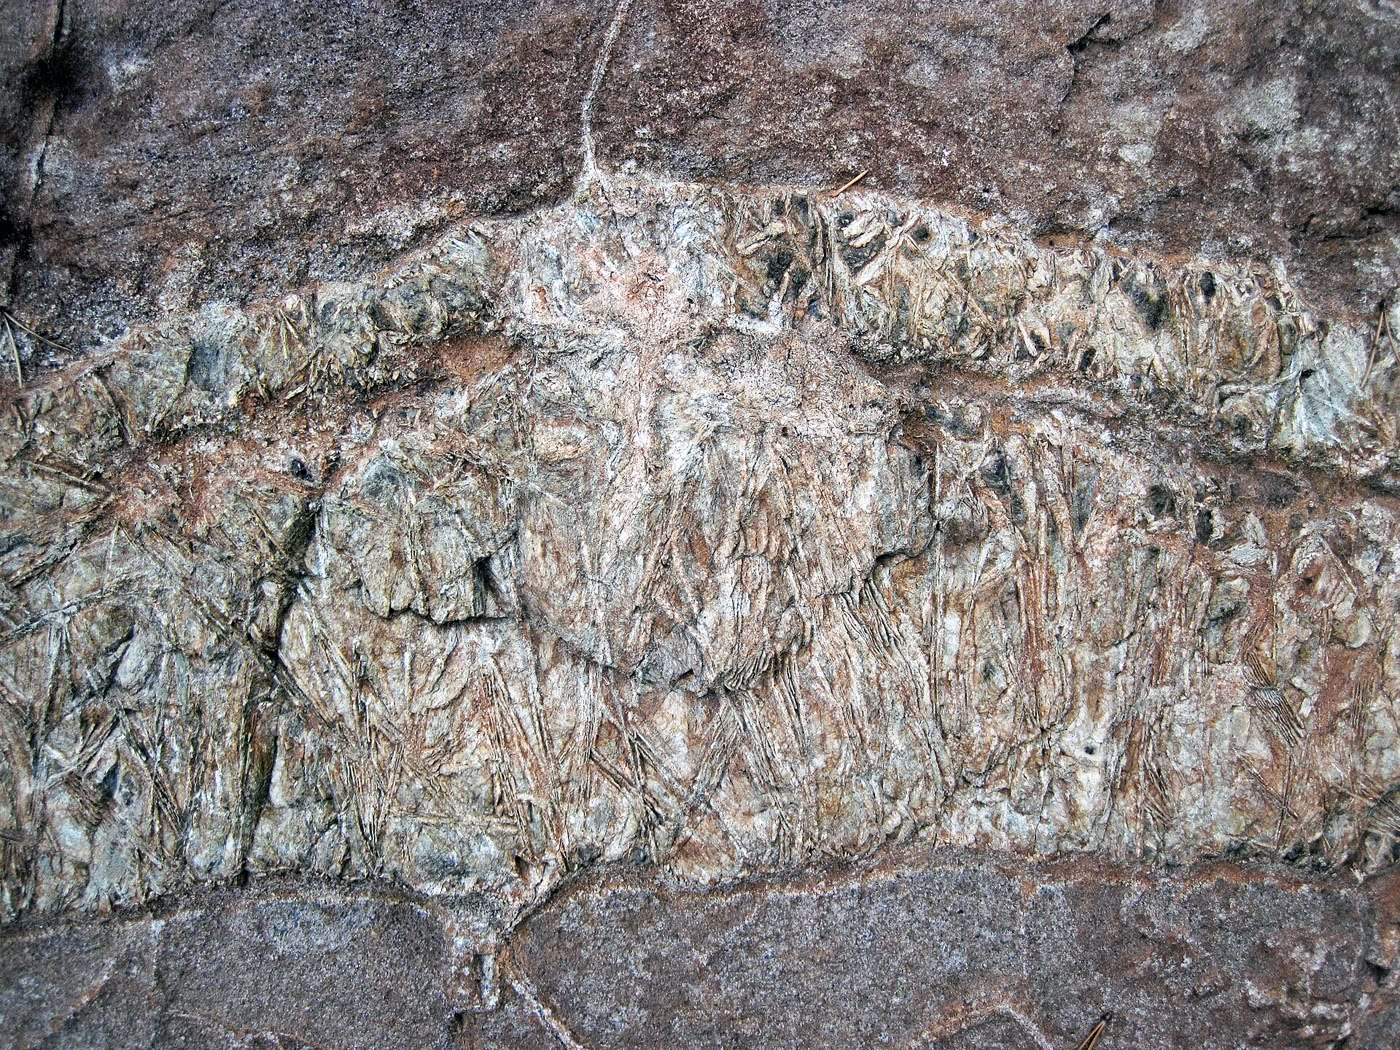
\includegraphics[width=0.66\linewidth]{images/book4/b2-18-spinifex-komatiite.jpg}
\par\smallskip{\small Textura spinifex num derrame de \omterm{def:b2:precambrian-earth:greenstone}{komatiito}, Pyke Hill, Ontário, parte de um
\omterm{def:b2:precambrian-earth:greenstone}{cinturão de rochas verdes} neoarqueano de cerca de 2.71 bilhões de anos: lâminas de olivina, hoje alteradas,
cresceram através do topo do derrame em resfriamento. Fotografia de James St.~John, CC~BY~2.0 (Wikimedia
Commons).}
\end{omfigure}

Os \omterm{def:b2:precambrian-earth:greenstone}{komatiitos} contêm até \qty{34}{\percent} de MgO, contra 10 a \qty{13}{\percent} nos basaltos
primários das dorsais atuais, e estão quase restritos à Terra antiga: o tipo empobrecido em alumínio
só se encontra em rochas com mais de \qty{2.8}{Ga}, o tipo não empobrecido em alumínio até cerca de
\qty{1.9}{Ga}, e só um tipo raro, enriquecido em alumínio, é tão jovem quanto \qty{90}{Myr}. Um fundido
tão rico em magnésio é muito quente e, como para os basaltos do
\cref{ch:b2:magmatic-differentiation}, o primeiro mineral a cristalizar dele é a olivina,
cuja proporção no líquido fixa a temperatura.
% ledger: pierru22:komatiite, asimow22:komatiite

\begin{proposition}[O termômetro dos komatiitos]\label{prop:b2:precambrian-earth:liquidus}
Para um fundido em equilíbrio com a olivina à pressão atmosférica, a temperatura do liquidus sobe
de modo quase linear com o teor de MgO do fundido. Por dois experimentos $(m_1, T_1)$ e
$(m_2, T_2)$,
\[
  T_{\text{liq}}(m) = T_1 + s\,(m - m_1), \qquad s = \frac{T_1 - T_2}{m_1 - m_2} .
\]
Experimentos de fusão em dois \omterm{def:b2:precambrian-earth:greenstone}{komatiitos}, $\qty{32.2}{\percent}$ de MgO a \qty{1616}{\celsius} e
$\qty{23}{\percent}$ a \qty{1450}{\celsius}, dão $s = \qty{18.0}{\celsius}$ por ponto percentual de
MgO.
\end{proposition}
% ledger: so16:liquidus, helz98:glass-thermometer

\begin{proof}
A olivina é uma solução sólida de forsterita e faialita, muito mais rica em magnésio que o fundido
do qual cresce. À medida que o fundido se resfria, a olivina retira-lhe magnésio, e a temperatura em
que o fundido está justamente saturado em olivina cai com seu teor de MgO. Os experimentos mostram que,
no intervalo de uma dada família de fundidos, a queda é quase linear, de modo que a reta por
dois experimentos interpola entre eles; $s = (1616 - 1450)/(32.2 - 23) = 166/9.2 = 18.04$.
\end{proof}

O coeficiente não é próprio dos \omterm{def:b2:precambrian-earth:greenstone}{komatiitos}. Vidros temperados da lava do Kilauea,
calibrados da mesma maneira, variam \qty{3}{\celsius} para \qty{0.15}{\percent} de MgO, ou
seja, \qty{20}{\celsius} por ponto percentual. Prolongar a reta dos \omterm{def:b2:precambrian-earth:greenstone}{komatiitos} até um basalto primário de dorsal
com \qty{12}{\percent} de MgO dá assim seu liquidus com uma margem de algumas dezenas de graus: $1616 -
18.0\times20.2 \approx \qty{1252}{\celsius}$. Os líquidos komatiíticos mais quentes eram, portanto,
uns \qty{360}{\celsius} mais quentes que os fundidos que alimentam as dorsais atuais, e a figura abaixo
mostra a reta.
% ledger: helz98:glass-thermometer, so16:liquidus, pierru22:komatiite
% values: slope 18.043, T_morb12 1251.5, dT_kom_morb 364.5 (precambrian.py)

\begin{omfigure}
\centering
\begin{tikzpicture}
\begin{axis}[omrecord, width=0.72\linewidth, height=6cm, xmin=8, xmax=35, ymin=1150, ymax=1700,
  xlabel={MgO no fundido (\unit{\percent} em massa)}, ylabel={liquidus a 1 atm (\unit{\celsius})},
  xtick pos=bottom, ytick pos=left, clip=false,
  y tick label style={/pgf/number format/1000 sep={}}]
% computed in figdata/bachelor-2/precambrian.py part kom; ledger: so16:liquidus, pierru22:komatiite
\fill[omProp!15] (axis cs:10,1150) rectangle (axis cs:13,1700);
\addplot[black, line width=1.1pt] table[x=MgO, y=T] {figdata/out/bachelor-2-precambrian-kom.dat};
\addplot[only marks, mark=*, mark size=2.4pt, omThm] coordinates {(32.2,1616) (23,1450)};
\node[anchor=north west, font=\scriptsize, text=omThm] at (axis cs:32.2,1612) {Barberton};
\node[anchor=north west, font=\scriptsize, text=omThm] at (axis cs:23,1446) {Munro};
\node[anchor=south, font=\scriptsize, text=omProp, align=center] at (axis cs:11.5,1560)
  {basaltos primários\\de dorsal};
\draw[densely dashed] (axis cs:12,1150) -- (axis cs:12,1251.5) -- (axis cs:8,1251.5);
\draw[densely dashed] (axis cs:32.2,1150) -- (axis cs:32.2,1616);
\draw[<->, omDef, thick] (axis cs:27,1251.5) -- (axis cs:27,1616);
\draw[densely dotted] (axis cs:12,1251.5) -- (axis cs:27,1251.5);
\draw[densely dotted] (axis cs:27,1616) -- (axis cs:32.2,1616);
\node[anchor=east, font=\scriptsize, text=omDef] at (axis cs:26.7,1330) {cerca de \qty{360}{\celsius}};
\end{axis}
\end{tikzpicture}
\par\smallskip{\small O termômetro dos \omterm{def:b2:precambrian-earth:greenstone}{komatiitos}: a reta pelas temperaturas do liquidus
medidas em dois \omterm{def:b2:precambrian-earth:greenstone}{komatiitos} (pontos), prolongada até os 10 a \qty{13}{\percent} de MgO dos basaltos
primários das dorsais atuais (faixa). O prolongamento apoia-se na inclinação semelhante dos fundidos basálticos.}
\end{omfigure}

Lava mais quente não significa um manto mais quente na mesma medida. Os \omterm{def:b2:precambrian-earth:greenstone}{komatiitos} provavelmente subiram em
plumas, como os basaltos mais quentes de hoje no Havaí, onde a temperatura potencial chega a
cerca de \qty{200}{\celsius} acima dos $1350 \pm \qty{50}{\celsius}$ do manto ambiente. E
formaram-se por altos graus de fusão, a maior profundidade. Considera-se em geral que se
formaram num manto de 200 a \qty{300}{K} mais quente que o atual; uma visão alternativa sustenta que
os \omterm{def:b2:precambrian-earth:greenstone}{komatiitos} eram \omterm{def:b2:magma-emplacement:magma}{magmas} hidratados, formados a temperaturas pouco mais altas que as do manto
circundante. De todo modo, o manto arqueano era mais quente, e os volumes
escolares deram uma razão: há 3 bilhões de anos os quatro isótopos radioativos liberavam mais do
dobro do calor atual (\cref{exo:b2:precambrian-earth:2}).
% ledger: asimow22:komatiite, pierru22:komatiite, so16:liquidus

\subsection*{TTG e o padrão de domos e quilhas}

Os gnaisses cinzentos entre os \omterm{def:b2:precambrian-earth:greenstone}{cinturões de rochas verdes} não são granitos do tipo que o
\cref{ch:b2:crustal-melting} descreveu.

\begin{definition}[Suíte tonalito--trondhjemito--granodiorito]\label{def:b2:precambrian-earth:ttg}
A \emph{suíte tonalito--trondhjemito--granodiorito}\index{suíte tonalito--trondhjemito--granodiorito}
(TTG) é a família de granitoides ricos em sódio e pobres em potássio --- tonalitos,
trondhjemitos (tonalitos pobres em minerais máficos) e granodioritos --- que forma a maior parte da
crosta continental arqueana. A maioria deles formou-se por \omterm{def:b2:mantle-melting:melting}{fusão parcial} de crosta basáltica
hidratada.
\end{definition}
% ledger: smithies19:ttg, cawood18:ttg

Boa parte do volume da crosta continental atual já se tinha formado no fim do \omterm{def:b2:precambrian-earth:eons}{Arqueano}, em grande parte
como TTG. Alguns TTG trazem assinaturas de \omterm{def:b2:elements-in-the-earth:trace}{elementos-traço} por muito tempo lidas como fusão a mais de
\qty{50}{km} de profundidade, uma pressão não atingida em crosta continental mais jovem, e essas leituras
pesam no debate sobre quando a tectônica de placas começou; um estudo de 2019 argumentou que essas assinaturas
vêm, na verdade, de fundidos do manto, e que os TTG comuns se formaram a
profundidades não maiores que os \qty{40}{km} de uma crosta continental comum de hoje. No fim do
\omterm{def:b2:precambrian-earth:eons}{Arqueano}, entre cerca de 3.0 e \qty{2.5}{Ga}, os granitoides da maioria dos \omterm{def:b2:precambrian-earth:craton}{crátons} passam de TTG
a granitos ricos em potássio, sinal de uma crosta mais espessa fundida de novo.
% ledger: smithies19:ttg, cawood18:ttg

No leste do Pilbara, na Austrália, no Zimbábue e no sul da Índia, os dois terrenos desenham um
padrão marcante no mapa. Domos arredondados de granitoide são emoldurados por quilhas sinclinais de rochas verdes cujas camadas mergulham e têm topo voltado para fora dos domos. Considera-se que os
domos subiram como \omterm{def:b2:magma-emplacement:ascent}{diápiros}, crosta granítica leve subindo através de uma pilha espessa e densa de
lavas que afundou entre eles. No Pilbara esse domeamento prosseguiu por centenas de milhões de
anos e parou há cerca de \qty{3.1}{Ga}, depois do que as estruturas se tornam lineares, como as
de \omterm{def:b2:alpine-orogen:orogen}{orógenos} mais jovens.
% ledger: cawood18:dome-keel

\begin{omfigure}
\centering
\begin{tikzpicture}[x=0.95cm, y=0.95cm, font=\scriptsize]
% schematic, after the description in cawood18:dome-keel
\fill[lith basalt] (0,0) rectangle (12,7);
\draw (0,0) rectangle (12,7);
\foreach \cx/\cy/\rx/\ry in {2.4/4.7/1.7/1.4, 7.2/5.0/2.0/1.4, 4.6/1.6/1.9/1.1, 10.0/2.0/1.4/1.3}
  \filldraw[lith granite, draw=black, thick] (\cx,\cy) ellipse ({\rx} and {\ry});
% strike and dip in the greenstone, each dipping away from the nearest dome
% (positions and strikes from the outward normals of the ellipses, computed by hand)
\foreach \px/\py/\st in {3.9/5.99/309, 0.9/5.99/231, 0.9/3.41/129, 2.4/2.88/90, 4.52/4.7/0,
    9.62/5.0/0, 8.91/6.29/305, 5.49/6.29/235, 8.91/3.71/55, 5.49/3.71/125,
    6.92/1.6/0, 4.6/3.12/270, 2.28/1.6/180, 6.24/0.53/60,
    10.0/3.72/270, 11.29/0.78/47, 8.18/2.0/180, 11.29/3.22/313}
  \pic at (\px,\py) {strikedip={\st}{}};
\node[fill=white, inner sep=1.5pt] at (2.4,4.7) {domo de TTG};
\node[fill=white, inner sep=1.5pt] at (7.2,5.0) {domo de TTG};
\node[fill=white, inner sep=1.5pt] at (4.6,1.6) {domo de TTG};
\node[fill=white, inner sep=1.5pt] at (10.0,2.0) {domo de TTG};
\node[fill=white, inner sep=1.5pt, align=center] at (7.45,2.75) {quilha de\\rochas verdes};
\node[fill=white, inner sep=1.5pt, align=center] at (1.0,0.9) {rochas verdes};
\pic at (11.4,5.6) {northarrow};
% section below
\begin{scope}[yshift=-3.3cm]
\fill[lith basalt] (0,0) -- (12,0) -- (12,2.2) -- (0,2.2) -- cycle;
\filldraw[lith granite, draw=black, thick] (0.6,0) .. controls (0.6,2.0) and (4.6,2.0) .. (4.6,0) -- cycle;
\filldraw[lith granite, draw=black, thick] (6.4,0) .. controls (6.4,2.1) and (11.0,2.1) .. (11.0,0) -- cycle;
\draw[thick] (0,0) rectangle (12,2.2);
\draw[black!70] (4.6,0.9) .. controls (5.5,0.2) .. (6.4,0.9);
\draw[black!70] (4.35,1.5) .. controls (5.5,0.6) .. (6.65,1.5);
\node[fill=white, inner sep=1.5pt] at (2.6,0.6) {TTG};
\node[fill=white, inner sep=1.5pt] at (8.7,0.6) {TTG};
\node[fill=white, inner sep=1.5pt] at (5.5,1.75) {quilha};
\draw[->, thick] (2.6,1.0) -- (2.6,1.75);
\draw[->, thick] (8.7,1.05) -- (8.7,1.8);
\draw[->, thick] (5.5,1.4) -- (5.5,0.95);
\node[anchor=west] at (12.1,1.1) {seção};
\end{scope}
\node[anchor=west] at (12.1,3.5) {mapa};
\end{tikzpicture}
\par\smallskip{\small O padrão de domos e quilhas de alguns \omterm{def:b2:precambrian-earth:craton}{crátons} arqueanos (esquemático, fora de
escala). Mapa: domos de granitoide da suíte TTG emoldurados por rochas verdes; os símbolos de direção e
mergulho mostram as camadas das rochas verdes mergulhando para fora de cada domo. Seção: os domos
sobem enquanto a pilha densa de rochas verdes afunda em quilhas sinclinais entre eles (setas).}
\end{omfigure}

\subsection*{Crátons}

\begin{definition}[Cráton]\label{def:b2:precambrian-earth:craton}
Um \emph{cráton}\index{cráton} é uma parte de um continente que se manteve tectonicamente estável
por mais de um bilhão de anos: um núcleo de crosta arqueana ou proterozoica, metamórfica e
plutônica, assentado sobre uma raiz espessa, fria e flutuante de manto litosférico que chega a uns
\qty{250}{km} de profundidade.
\end{definition}
% ledger: tulane:cratons, fischer:lithosphere, cawood18:ttg

Os \omterm{def:b2:precambrian-earth:craton}{crátons} estabilizaram-se sobretudo no Mesoarqueano e no Neoarqueano, e os sinais de sua
estabilidade estão escritos nas rochas: amplas bacias sedimentares depositadas sobre eles, como o
Supergrupo Transvaal sobre o \omterm{def:b2:precambrian-earth:craton}{cráton} de Kaapvaal (cerca de 2640 a \qty{2055}{Ma}) e o Supergrupo Mount Bruce
sobre o Pilbara (2775 a \qty{2210}{Ma}); enxames de \omterm{def:b2:magma-emplacement:bodies}{diques} retilíneos que os cortam como
placas rúpteis; e suas raízes espessas, adquiridas no fim do \omterm{def:b2:precambrian-earth:eons}{Arqueano}. Entre 3.2 e
\qty{2.5}{Ga} o registro mostra também as mais antigas margens passivas e \omterm{def:b2:alpine-orogen:foreland}{bacias de antepaís}, cinturões
de \omterm{def:b2:metamorphic-facies:metamorphism}{metamorfismo} pareados e evidências paleomagnéticas de que os \omterm{def:b2:precambrian-earth:craton}{crátons} se moviam uns em relação aos outros.
Uma revisão de 2018 lê essas mudanças como o início gradual da tectônica de placas tal como funciona
hoje, mas ressalta que nenhuma observação isolada o prova; as estimativas publicadas desse
início vão do \omterm{def:b2:precambrian-earth:eons}{Hadeano} ao Neoproterozoico.
% ledger: cawood18:transition, cawood18:ttg, cawood18:cratons

\begin{inthefield}[Ler um cinturão de rochas verdes]
Num \omterm{def:b2:precambrian-earth:greenstone}{cinturão de rochas verdes} a primeira pergunta que faz um geólogo que mapeia é para que lado era o topo quando as
rochas se formaram, já que as camadas são muitas vezes verticais ou invertidas. As lavas em almofada dão a resposta
por seus topos arredondados e pelas bases pontudas que enfiam nas almofadas de baixo; as camadas gradadas, por
sua granodecrescência para cima; e os derrames de \omterm{def:b2:precambrian-earth:greenstone}{komatiito}, por seu zoneamento: um topo resfriado e fraturado, com
lâminas spinifex crescendo para baixo nele, sobre uma base rica em cristais de olivina acumulados. As direções
de polaridade mapeadas estação por estação desenham os sinclinais das quilhas. Zircões de tufos félsicos
e dos TTG dos domos dão então idades U--Pb, de modo que o geólogo pode dizer quais
rochas verdes são mais antigas que os domos que hoje as atravessam.
\end{inthefield}
% ledger: so16:liquidus (spinifex in the top zones of flows), cawood18:dome-keel

\section{O oxigênio}\label{sec:b2:precambrian-earth:oxygen}

\subsection*{Um ar arqueano sem oxigênio}

A atmosfera primitiva dos volumes escolares era rica em nitrogênio e dióxido de carbono e
pobre em oxigênio. Indicadores e modelos hoje a delimitam com mais rigor. Antes de \qty{2.4}{Ga} o oxigênio
na superfície estava abaixo de um milionésimo do atual; o dióxido de carbono era talvez de 10 a 2500
vezes o atual e o metano de 100 a \num{10000} vezes. Grãos de uraninita e de pirita, que
o oxigênio destrói, foram carregados por rios arqueanos e depositados inalterados; a \qty{2.415}{Ga}
a sobrevivência de uraninita detrítica limita o oxigênio a \qty{3.2e-5}{atm}. O ciclo do carbono, lembrado
adiante, manteve a temperatura média da superfície entre cerca de 0 e \qty{40}{\celsius}.
% ledger: cz20:archean-air, kasting25:indicators

Oxigênio estava sendo produzido: as cianobactérias o liberam pela fotossíntese, e vestígios dele aparecem em
algumas rochas arqueanas. Mas ele era consumido tão depressa quanto se formava, pelos gases vulcânicos e pelo ferro
dissolvido no mar.
% ledger: luo16:goe, lyons21:boring

\begin{definition}[Formação ferrífera bandada]\label{def:b2:precambrian-earth:bif}
Uma \emph{formação ferrífera bandada}\index{formação ferrífera bandada} (BIF) é um sedimento químico de
finas camadas alternadas de óxidos de ferro --- hematita, magnetita --- e de chert. Ela precipita
da água do mar que carrega ferro(II) dissolvido, quando esse ferro é oxidado a
ferro(III) insolúvel; precisa, portanto, de um oceano profundo sem oxigênio, de um suprimento de ferro e de um oxidante
onde o ferro se deposita.
\end{definition}
% ledger: earle:bif, holland06:stages

As \omterm{def:b2:precambrian-earth:bif}{formações ferríferas bandadas} são mais abundantes de 2.4 a \qty{1.8}{Ga}; depois disso o oceano profundo
já não carregava ferro dissolvido suficiente, e elas praticamente desaparecem, para voltar brevemente nos
depósitos glaciais do Criogeniano (adiante). São um minério comum de ferro
(\cref{ch:b2:ore-deposits}).
% ledger: earle:bif, hoffman17:models

\subsection*{O Grande Evento de Oxidação}

\begin{definition}[Grande Evento de Oxidação]\label{def:b2:precambrian-earth:goe}
O \emph{Grande Evento de Oxidação}\index{Grande Evento de Oxidação} (GOE) é o intervalo, de cerca de
2.4--2.3 a cerca de \qty{2.1}{Ga}, durante o qual o oxigênio se acumulou pela primeira vez de modo duradouro na
atmosfera e no oceano raso, subindo de menos de um milionésimo de seu nível atual a
talvez um décimo.
\end{definition}
% ledger: cz20:goe, cz20:archean-air, gumsley17:goe, holland06:stages

O marcador mais claro é uma assinatura dos isótopos de enxofre. Nos sedimentos mais antigos que o GOE, os
isótopos do enxofre estão separados de um modo que só a fotoquímica num ar sem oxigênio
produz; a assinatura desaparece quando o oxigênio chega. Sua física e seu registro completo pertencem
ao volume do terceiro ano; aqui ela serve de relógio. Em três testemunhos de sondagem através do Supergrupo
Transvaal, na África do Sul, a assinatura some a \qty{2.33}{Ga}, em 1 a \qty{10}{Myr}:
a subida em si foi rápida. Outros registros situam o início do evento entre 2.46 e \qty{2.43}{Ga},
na época da primeira glaciação global, e mostram que o oxigênio não subiu de modo contínuo
depois.
% ledger: luo16:goe, farquhar00:sulfur, pk02:anoxic, gumsley17:goe

Depois do GOE aparecem as camadas vermelhas, a pirita e a uraninita detríticas desaparecem das areias fluviais,
e os solos retêm seu ferro como óxidos. Mas o oceano profundo continuou anóxico por mais de um bilhão
de anos.
% ledger: kasting25:indicators, lyons21:boring

\subsection*{O ``bilhão entediante'' e a segunda subida}

O intervalo de cerca de 1.8 a \qty{0.8}{Ga} mostra tão pouca variação nos isótopos de carbono dos
carbonatos marinhos que é amplamente chamado de ``bilhão entediante''. Seu oxigênio é debatido: as primeiras
estimativas davam de 1 a \qty{40}{\percent} do nível atual; os isótopos de cromo sugerem menos de
\qty{1}{\percent}, talvez \qty{0.1}{\percent}. O oceano profundo era anóxico. Ao longo desse intervalo
os eucariontes, como contam os livros de biologia, apareceram, se diversificaram e se multiplicaram. A partir de cerca de \qty{800}{Ma} muitos registros mostram
uma segunda subida, abrupta, do oxigênio, na época de grandes desenvolvimentos da vida complexa; se
o oxigênio os desencadeou ou os seguiu ainda se discute. Os grandes fósseis do Ediacarano
aparecem a partir de cerca de \qty{570}{Ma}. Enquanto isso, os \omterm{def:b2:wilson-cycle:supercontinent}{supercontinentes} do \cref{ch:b2:wilson-cycle}
se reuniram e se fragmentaram: as margens passivas, marca de fragmentação, são abundantes por volta de 2100 a
\qty{1850}{Ma}, quando Nuna se reuniu, e de novo de 650 a \qty{500}{Ma}.
% ledger: lyons21:boring, lyons21:eukaryotes, cawood18:ttg, nance22:supercontinents

\section{Gelo até o equador}\label{sec:b2:precambrian-earth:snowball}

\subsection*{A retroalimentação gelo--albedo}

A neve e o gelo refletem a maior parte da luz solar que recebem; o mar aberto, muito pouco: cerca de
\qty{6}{\percent} para o oceano, de 50 a \qty{70}{\percent} para o gelo marinho nu, até
\qty{90}{\percent} para o gelo coberto de neve. Uma Terra que se resfria forma mais gelo, reflete mais
luz solar e se resfria ainda mais.
% ledger: nsidc:albedo-ice, albedo:surfaces

\begin{definition}[Retroalimentação gelo--albedo]\label{def:b2:precambrian-earth:ice-albedo}
A \emph{retroalimentação gelo--albedo}\index{retroalimentação gelo--albedo} é a amplificação de uma variação
de temperatura pela variação da cobertura de neve e gelo que ela causa: o resfriamento estende o gelo, o que
aumenta o albedo do planeta, reduz a luz solar absorvida e resfria ainda mais o planeta;
o aquecimento funciona no sentido inverso. É uma retroalimentação positiva.
\end{definition}
% ledger: hoffman17:hysteresis, nsidc:albedo-ice

Suas consequências aparecem no modelo climático mais simples, um planeta de uma só temperatura $T$ e
capacidade térmica $C$ por metro quadrado. Ele absorve $\tfrac14 S(1 - a)$, onde $S$ é a luz solar
à sua distância e $a$ seu albedo, e perde a radiação de onda longa emitida do volume do
primeiro ano, escrita $\varepsilon\sigma T^4$: $\varepsilon$, a \emph{emissividade efetiva},
mede quanto da emissão da superfície escapa ao efeito estufa, e hoje vale
$240.2/(\sigma\times288^4) = 0.616$. Para incluir a retroalimentação, faz-se do albedo uma função da
temperatura. Este capítulo escolhe $a = 0.294$, o valor atual, quando $T \ge \qty{283}{K}$; $a
= 0.6$, o valor que os modelos climáticos dão a uma superfície globalmente congelada, quando $T \le \qty{263}{K}$; e
uma reta entre os dois. Os dois limiares são uma escolha de modelagem, não grandezas
medidas.
% ledger: earth:TSI, earth:albedo, earth:Tsurf, const:sigma, hoffman17:models
% values: eps 0.6158 (precambrian.py)

\begin{proposition}[Equilíbrios de um modelo de balanço de energia]\label{prop:b2:precambrian-earth:ebm}
No modelo
\[
  C\,\frac{\mathrm dT}{\mathrm dt} = \tfrac14 S\bigl(1 - a(T)\bigr) - \varepsilon\sigma T^4
  = R(T) - E(T),
\]
as temperaturas estacionárias são as soluções de $R(T) = E(T)$. Uma temperatura estacionária $T^*$ é
estável se $E'(T^*) > R'(T^*)$ e instável se $E'(T^*) < R'(T^*)$.
\end{proposition}

\begin{proof}
Numa solução de $R = E$ o lado direito se anula, de modo que $T$ não se move. Perto dela, ponha-se $T = T^*
+ \delta$: em primeira ordem $C\,\dot\delta = (R'(T^*) - E'(T^*))\,\delta$, cuja solução
$\delta(t) = \delta(0)\,e^{(R' - E')t/C}$ decai quando $E' > R'$ e cresce quando $E' < R'$.
\end{proof}

$E$ sempre cresce com $T$. $R$ é constante onde o albedo é fixo, de modo que os equilíbrios congelado e
quente são estáveis; na rampa entre eles $R$ cresce, porque o aquecimento derrete gelo, e, se
cresce mais depressa que $E$, um equilíbrio ali é instável. A figura abaixo mostra que, com a luz solar
atual, o modelo tem três equilíbrios.

\begin{example}[Três climas sob o Sol atual]\label{ex:b2:precambrian-earth:three}
Com $S_0 = \qty{1361}{W.m^{-2}}$, o equilíbrio quente é \qty{288}{K} por construção. Uma
bola de neve absorve $\tfrac14 S_0\times0.4 = \qty{136.1}{W.m^{-2}}$, de modo que $T^4 =
136.1/(0.616\,\sigma)$ e $T = \qty{249.8}{K}$, abaixo de \qty{263}{K}: o estado congelado também
existe. Entre os dois, na rampa, $R = E$ de novo a \qty{275.5}{K}, um estado instável: um
planeta um pouco mais quente aquece até \qty{288}{K}; um pouco mais frio congela.
\end{example}
% values: T_snow_today 249.9, T_mid_today 275.5 (precambrian.py)

\begin{omfigure}
\centering
\begin{tikzpicture}
\begin{axis}[omrecord, width=0.76\linewidth, height=6.2cm, xmin=215, xmax=305, ymin=80, ymax=280,
  xlabel={temperatura média global da superfície $T$ (\unit{K})}, ylabel={fluxo (\unit{W.m^{-2}})},
  xtick pos=bottom, ytick pos=left, clip=false,
  legend style={at={(0.5,1.04)}, anchor=south, draw=none, font=\scriptsize, legend columns=3}]
% computed in figdata/bachelor-2/precambrian.py part ebm; ledger: earth:TSI, earth:albedo, earth:Tsurf, const:sigma, hoffman17:models, gough81:luminosity
\fill[blue!8] (axis cs:263,80) rectangle (axis cs:283,280);
\addplot[black, line width=1.1pt, restrict x to domain=219:299] table[x=T_K, y=emit] {figdata/out/bachelor-2-precambrian-ebm.dat};
\addlegendentry{emitida $E(T)$}
\addplot[omThm, line width=1.1pt] table[x=T_K, y=absS0] {figdata/out/bachelor-2-precambrian-ebm.dat};
\addlegendentry{absorvida, Sol atual}
\addplot[omDef, line width=1.1pt, densely dashed] table[x=T_K, y=absP4] {figdata/out/bachelor-2-precambrian-ebm.dat};
\addlegendentry{absorvida, há 4 Ga}
\addplot[only marks, mark=*, mark size=2.4pt, black] coordinates {(249.9,136.1) (288,240.2)};
\addplot[only marks, mark=o, mark size=2.4pt, black, thick] coordinates {(275.5,204.4)};
\addplot[only marks, mark=*, mark size=2.4pt, omDef] coordinates {(231.8,100.85)};
\node[anchor=north west, font=\scriptsize] at (axis cs:250.5,134) {bola de neve};
\node[anchor=south east, font=\scriptsize] at (axis cs:287.5,242) {hoje};
\node[anchor=south east, font=\scriptsize] at (axis cs:275,206) {instável};
\node[anchor=north west, font=\scriptsize, text=omDef] at (axis cs:237,97.5) {o único estado há 4 Ga};
\node[anchor=north, font=\scriptsize, text=blue!60!black, align=center] at (axis cs:273,276)
  {o gelo\\recua};
\end{axis}
\end{tikzpicture}
\par\smallskip{\small O modelo de balanço de energia do texto: a radiação emitida (preto) e
a luz solar absorvida sob o Sol atual (vermelho) e sob o Sol de 4 bilhões de anos atrás,
com \qty{74}{\percent} do brilho (azul, tracejado), com a emissividade efetiva atual. Na faixa
sombreada o albedo cai de 0.6 para 0.294 à medida que o gelo recua. Pontos cheios: equilíbrios estáveis;
ponto vazio: instável.}
\end{omfigure}
% values: T_snow_4 231.8, lum_4 0.7406 (precambrian.py)

\begin{proposition}[Pontos de virada]\label{prop:b2:precambrian-earth:tipping}
Neste modelo o clima quente só existe se $S \ge S_{\text{f}}$ e a bola de neve só se
$S \le S_{\text{m}}$, onde
\[
  S_{\text{f}} = \frac{4\varepsilon\sigma T_2^4}{1 - a_{\text{w}}}, \qquad
  S_{\text{m}} = \frac{4\varepsilon\sigma T_1^4}{1 - a_{\text{i}}},
\]
sendo $T_1 = \qty{263}{K}$ e $T_2 = \qty{283}{K}$ as extremidades da rampa e $a_{\text{i}}$,
$a_{\text{w}}$ os albedos do planeta congelado e do planeta quente. Entre $S_{\text{f}}$ e
$S_{\text{m}}$ os dois existem.
\end{proposition}

\begin{proof}
No ramo quente $a = a_{\text{w}}$ e o equilíbrio é $T_{\text{w}} = (S(1 -
a_{\text{w}})/(4\varepsilon\sigma))^{1/4}$, que cresce com $S$; é um estado quente válido apenas
se $T_{\text{w}} \ge T_2$, isto é, $S \ge S_{\text{f}}$. Do mesmo modo, o equilíbrio de bola de neve
$(S(1 - a_{\text{i}})/(4\varepsilon\sigma))^{1/4}$ só é válido se não exceder $T_1$, isto
é, $S \le S_{\text{m}}$.
\end{proof}

Com a emissividade atual, $S_{\text{f}} = \qty{1269}{W.m^{-2}}$, \qty{93.2}{\percent} da luz solar
atual, e $S_{\text{m}} = \qty{1670}{W.m^{-2}}$, \qty{122.7}{\percent}. A figura abaixo
traça os equilíbrios em função da luz solar. Sua dobra forma um laço: uma Terra quente cuja luz solar
ou cujo efeito estufa se enfraquece além da dobra esquerda congela de uma vez, e uma Terra congelada continua congelada
até ser empurrada além da dobra direita, muito além das condições em que congelou. É
a histerese que Hoffman e colegas traçam para a Terra real com modelos mais completos,
com a linha do gelo avançando ``incontrolavelmente até o equador'' assim que atinge o limiar
de instabilidade.
% ledger: hoffman17:hysteresis
% values: S_freeze 1268.9, S_melt 1670.5, s_freeze 0.9323, s_melt 1.2274 (precambrian.py)

\begin{omfigure}
\centering
\begin{tikzpicture}
\begin{axis}[omrecord, width=0.76\linewidth, height=6.2cm, xmin=0.7, xmax=1.4, ymin=220, ymax=320,
  xlabel={luz solar $S/S_0$}, ylabel={temperatura de equilíbrio (\unit{K})},
  xtick pos=bottom, ytick pos=left, clip=false, unbounded coords=jump,
  x tick label style={/pgf/number format/.cd, fixed, fixed zerofill, precision=1}]
% computed in figdata/bachelor-2/precambrian.py part branch; ledger: earth:TSI, earth:albedo, earth:Tsurf, const:sigma, hoffman17:models, gough81:luminosity
\addplot[omDef, line width=1.2pt] table[x=s, y=Tsnow] {figdata/out/bachelor-2-precambrian-branch.dat};
\addplot[black, line width=1.0pt, densely dashed] table[x=s, y=Tmid] {figdata/out/bachelor-2-precambrian-branch.dat};
\addplot[omThm, line width=1.2pt] table[x=s, y=Twarm] {figdata/out/bachelor-2-precambrian-branch.dat};
\draw[black!50, densely dotted] (axis cs:1,220) -- (axis cs:1,320);
\draw[black!50, densely dotted] (axis cs:0.7406,220) -- (axis cs:0.7406,320);
\node[anchor=south west, font=\scriptsize, rotate=90] at (axis cs:1.0,222) {hoje};
\node[anchor=south west, font=\scriptsize, rotate=90] at (axis cs:0.7406,237) {há 4 Ga};
\draw[->, thick, blue!60!black] (axis cs:0.9323,281) -- (axis cs:0.9323,248);
\draw[->, thick, omThm] (axis cs:1.2274,265) -- (axis cs:1.2274,300);
\node[anchor=north west, font=\scriptsize, text=omThm] at (axis cs:1.02,314) {ramo quente};
\node[anchor=north, font=\scriptsize, text=omDef] at (axis cs:0.85,236) {ramo bola de neve};
\node[anchor=south, font=\scriptsize] at (axis cs:1.12,268) {instável};
\node[anchor=east, font=\scriptsize, text=blue!60!black, align=right] at (axis cs:0.925,266) {congela\\de uma vez};
\node[anchor=west, font=\scriptsize, text=omThm, align=left] at (axis cs:1.235,282) {degela\\de uma vez};
\end{axis}
\end{tikzpicture}
\par\smallskip{\small Os equilíbrios do modelo em função da luz solar, com a emissividade efetiva
atual: o ramo quente (vermelho), o ramo bola de neve (azul) e o ramo instável
entre eles (tracejado). As setas marcam os dois pontos de virada da
\cref{prop:b2:precambrian-earth:tipping}.}
\end{omfigure}

\subsection*{O Sol jovem fraco}

\begin{definition}[Problema do Sol jovem fraco]\label{def:b2:precambrian-earth:faint-sun}
O \emph{problema do Sol jovem fraco}\index{problema do Sol jovem fraco} é a contradição entre
os modelos do Sol, que o tornam de 25 a \qty{30}{\percent} mais fraco há \qty{4}{Ga}, e as
rochas, que mostram água líquida e um ciclo da água ativo ao longo do \omterm{def:b2:precambrian-earth:eons}{Arqueano}: com a atmosfera e o
albedo atuais, a Terra primitiva deveria estar congelada.
\end{definition}
% ledger: cz20:archean-air, feulner12:fys, gough81:luminosity

O modelo de balanço de energia torna o problema mais agudo do que os volumes escolares podiam. Com a lei de
Gough, a luz solar há \qty{4}{Ga} era \qty{74.1}{\percent} da atual, abaixo dos
\qty{93.2}{\percent} em que o clima quente desaparece: com a emissividade atual o único
equilíbrio é uma bola de neve a \qty{232}{K}. A lei só atinge $0.932$ há
\qty{0.83}{Gyr}. Durante mais de três quartos de sua história, portanto, a Terra com
o ar atual não poderia ter sido quente e, uma vez congelada, teria precisado de ainda mais para degelar.
% ledger: gough81:luminosity, connelly12:cai
% values: T_snow_4 231.8, ago_freeze 0.829 (precambrian.py)

\begin{example}[O efeito estufa da Terra jovem]\label{ex:b2:precambrian-earth:young-greenhouse}
Para manter \qty{288}{K} sob o Sol de \qty{4}{Ga} atrás com o albedo atual, a luz solar
absorvida é $0.741\times340.25\times0.706 = \qty{178.0}{W.m^{-2}}$, de modo que a emissividade efetiva
deve cair para $178.0/(\sigma\times288^4) = 0.456$, contra 0.616 hoje: a parcela da
emissão da superfície retida pelo efeito estufa deve subir de 0.384 para 0.544.
\end{example}
% values: eps_warm_4 0.456 (precambrian.py)

As rochas dizem que o efeito estufa era de fato mais forte. O dióxido de carbono sozinho teria bastado com
0.024 a \qty{1}{bar} dele há \qty{4}{Ga} e 0.004 a \qty{0.03}{bar} a \qty{2.5}{Ga}, e o
metano, abundante no ar anóxico, ajudou. Um termostato o manteve assim: o intemperismo dos silicatos,
que consome dióxido de carbono, desacelera quando o clima esfria e acelera quando aquece, de modo que o
dióxido de carbono do ar se ajusta até o clima ficar temperado. O mesmo termostato explica
como termina uma bola de neve.
% ledger: cz20:archean-air, feulner12:fys

\subsection*{A Terra bola de neve}

Os depósitos glaciais do Neoproterozoico --- diamictitos, pavimentos estriados, pedras caídas de
gelo flutuante em sedimento fino --- mostram mantos de gelo apoiados no fundo chegando ao mar em todas as latitudes,
e o paleomagnetismo, que o volume do terceiro ano trata, situa vários deles perto do equador. A glaciação Sturtiana,
por exemplo, começou numa paleolatitude de $21 \pm \ang{3}$\,N, no atual Yukon.
% ledger: hoffman17:cryochrons, hoffman17:ages, hoffman17:deposits

\begin{definition}[Terra bola de neve; carbonato de capa]\label{def:b2:precambrian-earth:snowball}
Uma \emph{Terra bola de neve}\index{Terra bola de neve} é um estado da Terra no qual o gelo cobre os
oceanos e os continentes até o equador, com mantos de gelo apoiados no fundo chegando ao mar em todas as
latitudes, durante milhões de anos. Um \emph{carbonato de capa}\index{carbonato de capa} é a camada de
rocha carbonática, tipicamente um dolomito claro e finamente laminado, que recobre bruscamente os depósitos
glaciais de uma bola de neve e registra seu fim súbito.
\end{definition}
% ledger: hoffman17:cryochrons, hoffman17:cap

\begin{omfigure}
\centering
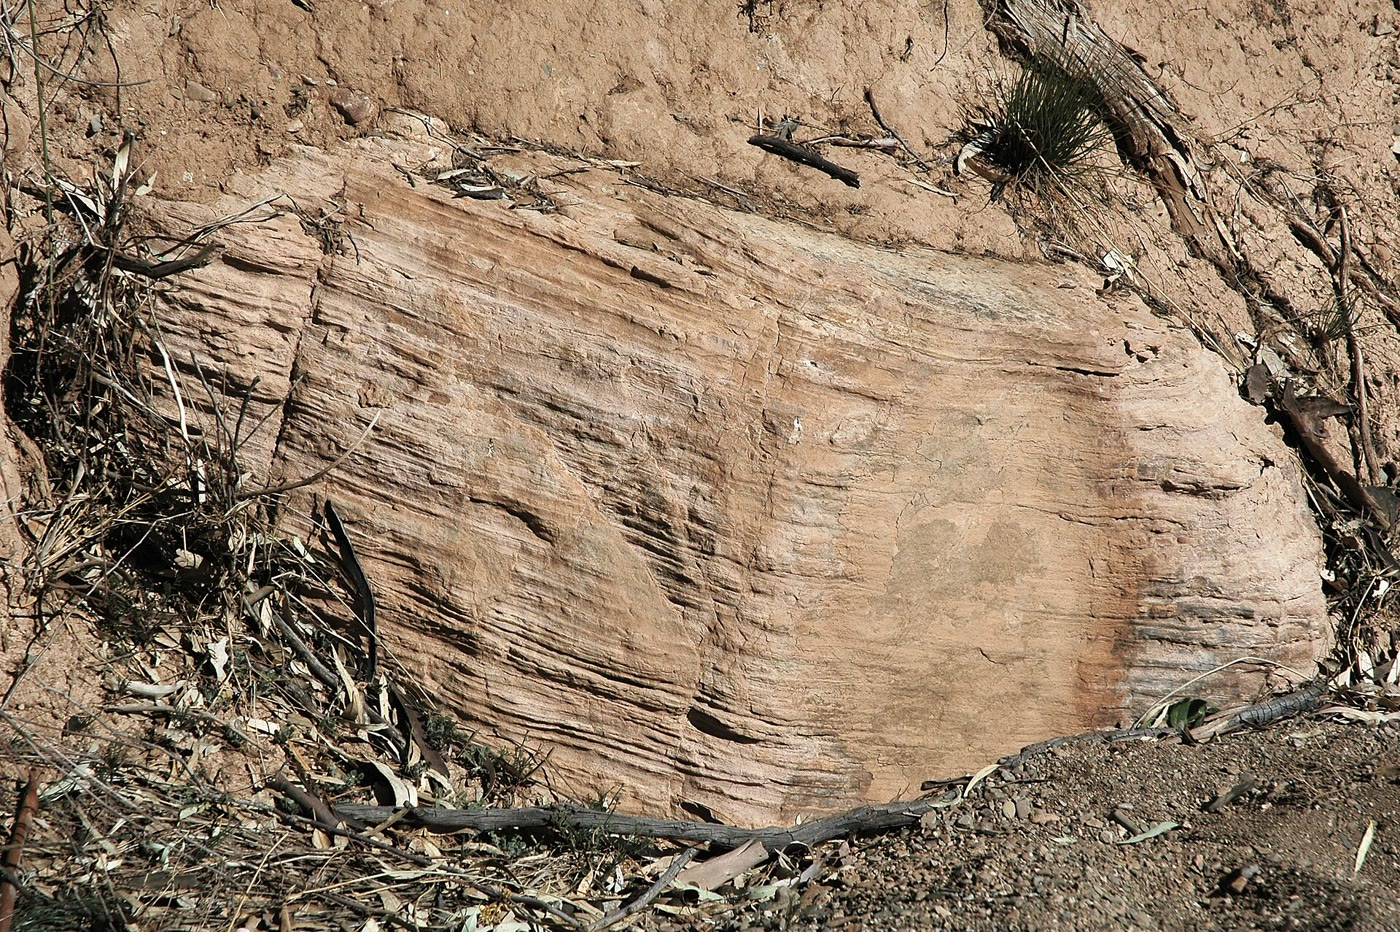
\includegraphics[width=0.66\linewidth]{images/book4/b2-18-cap-carbonate.jpg}
\par\smallskip{\small Um \omterm{def:b2:precambrian-earth:snowball}{carbonato de capa}: dolomito laminado da Formação Nuccaleena,
Flinders Ranges, Austrália Meridional, assentado sobre os depósitos da glaciação Marinoana
(as camadas estão inclinadas). Fotografia de James St.~John, CC~BY~2.0 (Wikimedia Commons).}
\end{omfigure}

Duas bolas de neve do Criogeniano estão hoje datadas por idades urânio--chumbo em zircões de cinzas
vulcânicas e por idades rênio--ósmio em folhelhos ricos em matéria orgânica. A Sturtiana começou entre 717.5 e
\qty{716.3}{Ma} e terminou entre 659.3 e \qty{658.5}{Ma}: \qty{58}{Myr} de gelo, com o
início e o fim sincrônicos no mundo inteiro. A Marinoana começou entre 649.9 e
\qty{639.0}{Ma}, mal datada, e terminou entre 636.0 e \qty{634.7}{Ma}: pelo menos
\qty{3}{Myr}. Cada uma termina com um único \omterm{def:b2:precambrian-earth:snowball}{carbonato de capa}, nunca com vários. As formações de ferro,
ausentes por um bilhão de anos, voltam nos depósitos glaciais sturtianos. Pelo menos uma bola de neve
anterior, no Sideriano, por volta de \qty{2.4}{Ga}, ocorreu na época do GOE; entre os dois
episódios, durante uns \qty{1.5}{Gyr}, quase nenhum manto de gelo é conhecido.
% ledger: hoffman17:ages, hoffman17:cryochrons, hoffman17:cap, hoffman17:models, hoffman17:earlier

\begin{history}[De uma hipótese estranha a uma teoria datada]
Em 1964 W.~B. Harland chamou a atenção para as evidências de uma glaciação do fim do Pré-Cambriano. Em
1968 e 1969 M.~I. Budyko, e W.~D. Sellers com um modelo semelhante, verificaram que a
\omterm{def:b2:precambrian-earth:ice-albedo}{retroalimentação gelo--albedo} podia fazer o gelo se espalhar até o equador uma vez que avançasse o bastante; uma
Terra globalmente congelada parecia então um estado sem volta e, portanto, um estado que nunca ocorrera.
Em 1981 J.~Walker, P.~Hays e J.~Kasting descreveram o termostato do intemperismo dos silicatos e
notaram que numa Terra congelada o dióxido de carbono dos vulcões se acumularia até o gelo
derreter: o estado podia terminar por si mesmo. Em 1992 J.~L. Kirschvink propôs que ele de fato
ocorrera e o chamou de ``Snowball Earth'' (\omterm{def:b2:precambrian-earth:snowball}{Terra bola de neve}); em 1998 P.~F. Hoffman e colegas publicaram
``A Neoproterozoic Snowball Earth'', e as épocas panglaciais passaram a ser chamadas de criocronos. Nenhum
depósito glacial criogeniano tinha sido datado radiometricamente antes de 2004; as datas acima são
obra dos anos seguintes.
\end{history}
% ledger: hoffman17:history

Os vulcões são a saída. Numa Terra coberta de gelo, a chuva e os rios quase param, e com eles o
intemperismo dos silicatos, e o dióxido de carbono que os vulcões liberam se acumula no ar
até que seu efeito estufa derreta o gelo.

\begin{proposition}[Acúmulo de dióxido de carbono]\label{prop:b2:precambrian-earth:co2}
Se o dióxido de carbono é liberado a uma taxa $F$ (massa por ano) numa atmosfera de massa
$M_{\text{a}}$ e massa molar média $\bar M$, sem sumidouro, o tempo necessário para levar sua fração molar
(razão de mistura em volume) de quase zero a $x$ é
\[
  \tau = \frac{x}{1 - x}\,\frac{M_{\mathrm{CO_2}}}{\bar M}\,\frac{M_{\text{a}}}{F} .
\]
\end{proposition}

\begin{proof}
A atmosfera contém $n = M_{\text{a}}/\bar M$ mols dos outros gases. Acrescentar $n_c$ mols de
dióxido de carbono torna sua razão de mistura $x = n_c/(n + n_c)$, de modo que $n_c = n\,x/(1 - x)$, de massa
$n_c M_{\mathrm{CO_2}}$; à taxa $F$ isso leva $\tau = n_c M_{\mathrm{CO_2}}/F$.
\end{proof}

\begin{example}[Quanto tempo para escapar?]\label{ex:b2:precambrian-earth:escape}
A maior das estimativas preferidas da liberação vulcânica atual é de \qty{0.26}{Gt} de dióxido
de carbono por ano. As estimativas da
razão de mistura necessária para terminar uma bola de neve criogeniana vão de 0.01 a 0.1. Com $M_{\text{a}} =
\qty{5.1e18}{kg}$, $\bar M = \qty{28.97}{g.mol^{-1}}$ e $M_{\mathrm{CO_2}} =
\qty{44.01}{g.mol^{-1}}$, $x = 0.01$ leva $\frac{0.01}{0.99}\times1.519\times\qty{5.1e18}{kg}
/ \qty{0.26e12}{kg.yr^{-1}} = \qty{0.30}{Myr}$, e $x = 0.1$ leva \qty{3.3}{Myr}.
\end{example}
% ledger: usgs:volcanic-co2, hoffman17:co2, earth:Matm, earth:Mmol, ciaaw:abridged-2024
% values: co2_t001_Myr 0.301, co2_t01_Myr 3.311 (precambrian.py)

Uma coluna de dióxido de carbono puro pesando \qty{1}{bar} sobre a Terra inteira levaria
\qty{20}{Myr} à mesma taxa, o número que Walker, Hays e Kasting deram. Alguns milhões de anos
é muito tempo, mas a Sturtiana durou \qty{58}{Myr}. Ou o limiar era mais alto, ou a
desgaseificação menor, ou a Terra congelada ainda tinha sumidouros: o intemperismo do fundo oceânico jovem,
que não para sob o gelo, é um candidato. No modelo de balanço de energia, a saída exige
que a emissividade efetiva da bola de neve caia até sua temperatura atingir \qty{263}{K}: sob
o Sol criogeniano, com \qty{94}{\percent} do atual, de 0.616 para 0.472, uma retenção extra de
uns \qty{39}{W.m^{-2}} (\cref{exo:b2:precambrian-earth:10}).
% ledger: hoffman17:co2, hoffman17:models, usgs:volcanic-co2
% values: one_bar_Myr 19.98, eps_melt_094 0.4716, forcing_melt_094 39.1 (precambrian.py)

Quando o gelo finalmente se abre no equador, a retroalimentação funciona ao contrário: o mar escuro absorve mais
luz solar, o gelo recua, e os modelos fazem a linha do gelo correr para os polos em cerca de
\qty{2}{kyr}. A Terra se vê então com um efeito estufa enorme sobre uma superfície escura, um
rescaldo quente. O intemperismo, muito rápido nesse clima, despeja cálcio, magnésio e bicarbonato no
mar, onde os \omterm{def:b2:precambrian-earth:snowball}{carbonatos de capa} precipitam enquanto a água de degelo inunda as plataformas; são precisos
uns dez milhões de anos para fazer o dióxido de carbono baixar de novo. Os mantos de gelo e os \omterm{def:b2:precambrian-earth:snowball}{carbonatos
de capa}, as formações de ferro e as idades sincrônicas são a razão pela qual a maioria dos geólogos hoje aceita
que as bolas de neve criogenianas ocorreram, embora quão severas foram --- se uma faixa de água
aberta sobreviveu no equador, como propõem os modelos de ``cinturão de água'' (waterbelt) --- ainda se discuta.
% ledger: hoffman17:hysteresis, hoffman17:cap, hoffman17:debate

\section*{Exercícios}\label{sec:b2:precambrian-earth:exercises}

Dados para os exercícios, salvo indicação em contrário: $\sigma = \qty{5.670e-8}{W.m^{-2}.K^{-4}}$;
$S_0 = \qty{1361}{W.m^{-2}}$; albedo atual 0.294 e temperatura média da superfície \qty{288}{K};
albedo da bola de neve 0.6; rampa de \qty{263}{K} a \qty{283}{K}; emissividade efetiva atual
0.616; lei de Gough $L/L_0 = 1/(1 + 0.4\,t/t_\odot)$ para um tempo $t$ antes do presente, $t_\odot =
\qty{4.567}{Gyr}$; liquidus dos \omterm{def:b2:precambrian-earth:greenstone}{komatiitos} \qty{1616}{\celsius} a \qty{32.2}{\percent} de MgO,
inclinação \qty{18.0}{\celsius} por ponto percentual; meias-vidas \ce{^{238}U} \qty{4.468}{Gyr}, \ce{^{235}U}
\qty{0.704}{Gyr}, \ce{^{232}Th} \qty{14.0}{Gyr}, \ce{^{40}K} \qty{1.248}{Gyr}.
% ledger: const:sigma, earth:TSI, earth:albedo, earth:Tsurf, hoffman17:models, gough81:luminosity, connelly12:cai, so16:liquidus, iaea:isotopes

\begin{exercise}[$\star$]\label{exo:b2:precambrian-earth:1}
(a) Quanto duraram o \omterm{def:b2:precambrian-earth:eons}{Hadeano}, o \omterm{def:b2:precambrian-earth:eons}{Arqueano} e o \omterm{def:b2:precambrian-earth:eons}{Proterozoico}? (b) Que fração da idade
da Terra os três juntos representam? (c) Que idade tinha a Terra quando cristalizou o zircão mais antigo
conhecido e quando se formaram as rochas mais antigas?
\end{exercise}

\begin{exercise}[$\star$]\label{exo:b2:precambrian-earth:2}
Hoje a \omterm{def:b2:elements-in-the-earth:bse}{Terra silicática total} libera, por quilograma, \qty{1.917}{pW} do \ce{^{238}U},
\qty{0.082}{pW} do \ce{^{235}U}, \qty{2.089}{pW} do \ce{^{232}Th} e \qty{0.818}{pW} do
\ce{^{40}K} ($\qty{1}{pW} = \qty{e-12}{W}$). (a) Calcule cada contribuição há \qty{3}{Gyr}, e
o total. (b) Por que fator a produção de calor caiu desde então? (c) Que isótopo lidera
hoje, e qual liderava então?
\end{exercise}

\begin{exercise}[$\star$]\label{exo:b2:precambrian-earth:3}
Use o termômetro dos \omterm{def:b2:precambrian-earth:greenstone}{komatiitos}. (a) Qual é o liquidus de um \omterm{def:b2:precambrian-earth:greenstone}{komatiito} com
\qty{28}{\percent} de MgO? (b) Que teor de MgO corresponde a \qty{1500}{\celsius}? (c) Um
derrame com textura spinifex tem MgO de rocha total de \qty{38}{\percent}. Por que seu liquidus não
deve ser lido na reta?
\end{exercise}

\begin{exercise}[$\star$]\label{exo:b2:precambrian-earth:4}
Ponha em ordem e dê as idades aproximadas de: o \omterm{def:b2:precambrian-earth:goe}{Grande Evento de Oxidação}, os
primeiros estromatólitos, o fim da glaciação Marinoana, os últimos \omterm{def:b2:precambrian-earth:greenstone}{komatiitos} comuns, as
rochas mais antigas, a segunda subida do oxigênio, os primeiros fósseis ediacaranos, o fim das estruturas
de domos e quilhas do Pilbara.
\end{exercise}

\begin{exercise}[$\star\star$]\label{exo:b2:precambrian-earth:5}
(a) Verifique que a emissividade efetiva da Terra atual é 0.616. (b) Calcule o equilíbrio de
bola de neve sob o Sol atual. (c) Mostre que o equilíbrio intermediário, \qty{275.5}{K}, satisfaz
$R = E$ com margem de \qty{0.5}{W.m^{-2}}. (d) Calcule as inclinações de $R$ e de $E$ ali, e conclua
que ele é instável.
\end{exercise}

\begin{exercise}[$\star\star$]\label{exo:b2:precambrian-earth:6}
(a) Usando a lei de Gough, calcule a luz solar há \qty{2.4}{Ga} e há \qty{0.65}{Ga} como frações
da atual. (b) No modelo, é possível um clima quente em cada data com a emissividade atual?
(c) Hoffman e colegas escrevem que o Sol sideriano era cerca de \qty{10}{\percent} mais fraco que
o Sol criogeniano. Verifique.
\end{exercise}

\begin{exercise}[$\star\star$]\label{exo:b2:precambrian-earth:7}
A Sturtiana durou de \qty{716.9}{Ma} a \qty{658.9}{Ma} (meios dos intervalos datados),
a Marinoana de \qty{644.5}{Ma} a \qty{635.4}{Ma}. (a) Calcule suas durações e o
interglacial entre elas. (b) Que fração do período Criogeniano, de 720 a \qty{635}{Ma},
o gelo cobriu a Terra, segundo esses números? (c) Por que a duração da Marinoana é só um
valor aproximado?
\end{exercise}

\begin{exercise}[$\star\star$]\label{exo:b2:precambrian-earth:8}
(a) Quanto tempo levam os vulcões, a \qty{0.26}{Gt} por ano e sem sumidouro, para levar o ar a
uma razão de mistura de dióxido de carbono de 0.05? (b) Quantas vezes as \qty{278}{ppm} de 1750 isso representa? (c) Se metade da liberação fosse absorvida pelo intemperismo do fundo
oceânico, quanto tempo levaria?
\end{exercise}
% ledger: usgs:volcanic-co2, earth:Matm, earth:Mmol, ciaaw:abridged-2024, ipcc:erf-2xco2

\begin{exercise}[$\star\star$]\label{exo:b2:precambrian-earth:9}
Um diamictito neoproterozoico contém pedras estriadas, algumas das quais repousam sobre lama finamente laminada
que está encurvada para baixo sob elas. (a) O que indica o encurvamento? (b) Sua paleolatitude é
\ang{10}. Por que isso importa para a hipótese da bola de neve? (c) Ele é recoberto diretamente por um
dolomito laminado rosado de alguns metros de espessura. O que é, e o que registra?
\end{exercise}

\begin{exercise}[$\star\star\star$]\label{exo:b2:precambrian-earth:10}
Sob o Sol criogeniano, $S = 0.94\,S_0$. (a) Mostre que no modelo o estado quente ainda
existe, por pouco, mas que uma bola de neve também existe. (b) Calcule a temperatura da bola de neve com
a emissividade atual. (c) Calcule a emissividade na qual a bola de neve atinge \qty{263}{K} e
degela. (d) Converta a variação de emissividade numa retenção extra de radiação de onda longa a
\qty{263}{K}, em \unit{W.m^{-2}}.
\end{exercise}

\begin{exercise}[$\star\star\star$]\label{exo:b2:precambrian-earth:11}
(a) Usando os pontos de virada da \cref{prop:b2:precambrian-earth:tipping}, mostre que a largura
do laço de histerese, $S_{\text{m}}/S_{\text{f}}$, não depende da emissividade, e
calcule-a. (b) O que tornaria o laço mais estreito? (c) Por que uma bola de neve só pode degelar longe
das condições em que congelou?
\end{exercise}

\begin{exercise}[$\star\star\star$]\label{exo:b2:precambrian-earth:12}
Deduza a constante de tempo do modelo de balanço de energia perto do equilíbrio quente, $\tau =
C/(E'(T^*) - R'(T^*))$, e calcule-a para uma camada de mistura oceânica de \qty{50}{m} de profundidade, de densidade
\qty{1025}{kg.m^{-3}} e calor específico \qty{3992}{J.kg^{-1}.K^{-1}}. O que acontece com $\tau$ quando a
luz solar se aproxima do ponto de virada esquerdo, neste modelo e num modelo cujo albedo varia
suavemente com a temperatura?
\end{exercise}
% ledger: noaa:seawater-1025, teos10:cp0

\begin{problem}[{Problema de fim de semana --- uma Terra jovem mais quente}]\label{pb:b2:precambrian-earth:1}
Este problema acompanha a Terra jovem de seu interior até seu ar. Use os dados dos
exercícios; a \omterm{def:b2:elements-in-the-earth:bse}{Terra silicática total} contém \qty{0.0203}{ppm} de urânio, \qty{0.0795}{ppm} de
tório e \qty{240}{ppm} de potássio em massa, e seus isótopos liberam \qty{95.13}{\micro W}
(\ce{^{238}U}), \qty{568.47}{\micro W} (\ce{^{235}U}), \qty{26.28}{\micro W} (\ce{^{232}Th}) e
\qty{28.47}{\micro W} (\ce{^{40}K}) por quilograma de isótopo. Em massa, o urânio é
\qty{99.29}{\percent} \ce{^{238}U} e \qty{0.711}{\percent} \ce{^{235}U}, e o potássio
\qty{0.0120}{\percent} \ce{^{40}K}. Arredonde a três algarismos significativos.

\noindent\textbf{Parte I --- O calor do interior.}
\begin{enumerate}
  \item Calcule o calor liberado hoje por cada isótopo por quilograma de \omterm{def:b2:elements-in-the-earth:bse}{Terra silicática total}, em
        \unit{pW.kg^{-1}}.
  \item Calcule o total.
  \item Calcule a constante de decaimento de cada isótopo, em \unit{Gyr^{-1}}.
  \item Calcule cada contribuição há \qty{2.7}{Gyr}, quando os \omterm{def:b2:precambrian-earth:greenstone}{komatiitos} de Pyke Hill extravasaram.
  \item Calcule o total então, e a razão em relação ao atual.
  \item Que isótopo dava mais calor então? Por que dá tão pouco hoje?
\end{enumerate}

\noindent\textbf{Parte II --- O Sol do Arqueano.}
\begin{enumerate}[resume]
  \item Com a lei de Gough, calcule a luz solar há \qty{2.7}{Ga} como fração da atual, e em
        \unit{W.m^{-2}}.
  \item Calcule o equilíbrio quente com essa luz solar e a emissividade atual. É um estado quente
        válido do modelo?
  \item Calcule o equilíbrio de bola de neve com essa luz solar.
  \item Que emissividade efetiva manteria a Terra a \qty{288}{K} com o albedo quente?
  \item O dióxido de carbono sozinho poderia tê-lo feito com 0.004 a \qty{0.03}{bar} a \qty{2.5}{Ga}.
        Numa atmosfera de cerca de \qty{1}{bar}, quantas vezes as \qty{278}{ppm} de 1750
        isso representa?
  \item Nomeie o processo que manteve o dióxido de carbono nesse nível durante centenas de milhões
        de anos.
\end{enumerate}

\noindent\textbf{Parte III --- Uma bola de neve e seu fim.}
\begin{enumerate}[resume]
  \item A primeira bola de neve, há \qty{2.4}{Ga}: calcule a luz solar então como fração da atual.
        O estado quente do modelo ainda é possível com a emissividade atual?
  \item A \qty{0.26}{Gt} de dióxido de carbono por ano, quanto tempo leva para atingir uma razão
        de mistura de 0.1?
  \item Se o limiar sob o Sol sideriano mais fraco fosse o dobro, 0.2, quanto tempo?
  \item Que rocha registra o fim de uma bola de neve, e como?
  \item Por que as formações de ferro da Sturtiana precisam de um oceano sem oxigênio sob o gelo?
\end{enumerate}

\noindent\textbf{Parte IV --- O termômetro dos komatiitos.}
\begin{enumerate}[resume]
  \item Verifique a inclinação da reta dos \omterm{def:b2:precambrian-earth:greenstone}{komatiitos} a partir dos dois experimentos.
  \item Um líquido komatiítico de Pyke Hill tinha \qty{30}{\percent} de MgO. Calcule seu liquidus.
  \item Calcule o liquidus do \omterm{def:b2:precambrian-earth:greenstone}{komatiito} de Barberton, \qty{32.2}{\percent} de MgO.
  \item Calcule o liquidus de um basalto primário de dorsal com \qty{12}{\percent} de MgO.
  \item Com a inclinação do Kilauea, \qty{20}{\celsius} por ponto percentual, em vez disso, quão quente seria o
        basalto, partindo do ponto de Barberton? Quanto importa a escolha da inclinação?
  \item Por que a diferença de temperatura entre as duas lavas é maior que a diferença de
        temperatura potencial entre o manto arqueano e o atual?
  \item Em resumo: quanto a lava komatiítica arqueana mais quente era mais quente que um basalto primário
        das dorsais atuais?
\end{enumerate}
\end{problem}
% ledger: ms95:pm-trace, dye:isotope-heat, iaea:isotopes, gough81:luminosity, cz20:archean-air, ipcc:erf-2xco2, usgs:volcanic-co2, hoffman17:co2, so16:liquidus, helz98:glass-thermometer, pierru22:komatiite
